


\documentclass{standalone}

%\pgfplotsset{compat=1.3}
%\usepgfplotslibrary{fillbetween}
\usepackage{comment}

\begin{comment}
#--------------------------------------------------------------------------
#Copyright (c) 2016 by Abdullah Al-Dujaili
#
#This file is part of EmbeddedHunter - large-scale black-box solver
#EmbeddedHunter is free software: you can redistribute it and/or modify it under
#the terms of the GNU General Public License as published by the Free
#Software Foundation, either version 3 of the License, or (at your option)
#any later version.
#
#EmbeddedHunter is distributed in the hope that it will be useful, but WITHOUT
#ANY WARRANTY; without even the implied warranty of MERCHANTABILITY or
#FITNESS FOR A PARTICULAR PURPOSE.  See the GNU General Public License for
#more details.
#
#You should have received a copy of the GNU General Public License along
#with EmbeddedHunter.  If not, see <http://www.gnu.org/licenses/>.
#--------------------------------------------------------------------------
#Author information
#Abdullah Al-Dujaili
#ash.aldujaili@gmail.com
#--------------------------------------------------------------------------
\end{comment}


\usepackage{multirow}
\usepackage{booktabs}
\usepackage{pgfplots,tikz}
\usepackage{pgfkeys}
\usepackage{pgfplotstable}
\usetikzlibrary{spy}
\usetikzlibrary{backgrounds}
%\usepackage{etoolbox}

\definecolor{c1}{rgb}{0.83, 0.0, 0.25}
\definecolor{c2}{rgb}{1.0, 0.44, 0.37}
\definecolor{c3}{rgb}{0.84, 0.23, 0.24}
\definecolor{c4}{rgb}{0.15, 0.38, 0.61}
\definecolor{c6}{rgb}{0.0, 0.56, 0.0}
%\usepackage{ifthen}


%legend columns=3,legend style={align=center,draw=none,column sep=2ex},

% for legend
% argument #1: any options
\newenvironment{customlegend}[1][]{%
	\begingroup
	% inits/clears the lists (which might be populated from previous
	% axes):
	\csname pgfplots@init@cleared@structures\endcsname
	\pgfplotsset{#1}%
}{%
% draws the legend:
\csname pgfplots@createlegend\endcsname
\endgroup
}%

% makes \addlegendimage available (typically only available within an
% axis environment):
\def\addlegendimage{\csname pgfplots@addlegendimage\endcsname}


% for plot entries
\newcommand{\plottikz}[5]{
	
	
	\pgfplotstableread{./fig/exp-#1-pid-#2.table}{\table}
	\begin{minipage}{\textwidth}
		%	\vspace{2em}
		\resizebox{1.\textwidth}{!}{
	%	\hspace{1em}
		\begin{tikzpicture}
		%ymax  =1, xmin=1,xmax=1e3 \#\texttt{fevals}
		\begin{axis}[ymode=#5,xmode=#4, xlabel=#3, ylabel=\texttt{regret},legend style={at={(0.25,-0.5)},anchor=east}]

		\addplot[densely dashed,thick, black, mark=diamond, mark options ={black, solid},mark size=4pt,samples=10]  table [x=at, y=RESOO,col sep=tab]{\table};
		\addplot[solid, draw = black, thick,mark=asterisk,samples=10]  table [x=at, y=SRESOO,col sep=tab]{\table};
		\addplot[densely dotted, draw = black,thick, mark options={black,solid}, mark=square,mark size=3pt,samples=20]  table [x=at, y=EmbeddedHunter,col sep=tab]{\table};
    %	\addplot[solid, draw = c1,thick, mark= square,samples=10]  table [x=at, y=RandomSearch]{\table};
%		\addplot[solid, draw = red, thick,mark=triangle, samples=10]  table [x=at, y=SRECMA]{\table};

%		\addlegendentry{\texttt{\textsc{EmbeddedHunter}}}
%		\addlegendentry{\texttt{RESOO}}
%		\addlegendentry{\texttt{SRESOO}}


	%	\addlegendentry{\texttt{RECMA}}
%		\addlegendentry{\texttt{SRECMA}}
		\end{axis}
		\end{tikzpicture}
			%\hspace{1em}
%	
}
%\vspace{2em}
\end{minipage}

}


\newcommand{\problemname}[2]{
	\begin{minipage}{0.75\textwidth}
	\textbf{\textit{\Large #1}} \\
	\textbf{\large #2}
	\end{minipage}
	}

\begin{document}




\begin{tabular}{|ll||l|l|l|l|}
	\toprule
	% top column algorithms and problems
	&\Large	\textbf{Algorithms}

	& \multicolumn{4}{c|}{\Large \textbf{Problems}} \\
	%\cmidrule{1-1}
    &
    % algorithm description and problems
\begin{minipage}{0.25\textwidth}
	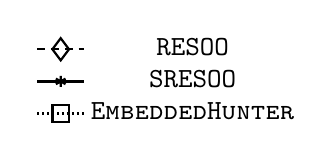
\begin{tikzpicture}[]
		\begin{customlegend}[legend style={align=left,draw=none},legend entries={\texttt{\textsc{RESOO}},\texttt{\textsc{SRESOO}},\texttt{\textsc{EmbeddedHunter}}}]
		\addlegendimage{densely dashed,thick, black, mark=diamond, mark options ={black, solid},mark size=4pt} 
		\addlegendimage{solid, draw = black, thick,mark=asterisk}
		\addlegendimage{densely dotted, draw = black,thick, mark options={black,solid}, mark size=3pt,mark=square}
		\end{customlegend}
	\end{tikzpicture}
\end{minipage}
	& \multicolumn{1}{l|}{\problemname{Ellipsoid}{ill-conditioned, uni-modal, separable}} & 
	\problemname{FletcherPowell}{periodic search space, multi-modal, non-separable} & 
	\problemname{Rosenbrock}{non-convex, uni-modal, non-separable} & 
	\problemname{Ackley} {$|$local minima$|$ $\in \mathcal{O}(e^n)$, non-separable} \\
	\midrule
	\midrule
	% Experiments
	\multirow{4}{*}{\rotatebox[origin=c]{90}{\bf \Large Experiments \hspace{26em}}}
	&\textit{\textbf{\Large Convergence ($v$)}} & \plottikz{3}{1}{$v$}{log}{log}& \plottikz{3}{2}{$v$}{log}{log} &  \plottikz{3}{6}{$v$}{log}{linear} & \plottikz{3}{8}{$v$}{log}{log} \\ \cmidrule{2-6}
	
	&\textit{\textbf{\Large  Scalability ($n$)}} & \plottikz{2}{1}{$n$}{log}{log}& \plottikz{2}{2}{$n$}{log}{log} &  \plottikz{2}{6}{$n$}{log}{linear} & \plottikz{2}{8}{$n$}{log}{log} \\ \cmidrule{2-6}
	
	&\textit{\textbf{\Large Embeddings Number ($M$)}} & \plottikz{0}{1}{$M$}{linear}{log}& \plottikz{0}{2}{$M$}{linear}{log} &  \plottikz{0}{6}{$M$}{linear}{linear} & \plottikz{0}{8}{$M$}{linear}{log} \\ \cmidrule{2-6}
	
	&\textit{\textbf{\Large Effective Dimension ($d$)}} &  \plottikz{1}{1}{$d$}{linear}{log}& \plottikz{1}{2}{$d$}{linear}{log} &  \plottikz{1}{6}{$d$}{linear}{log} & \plottikz{1}{8}{$d$}{linear}{log} \\
	\cmidrule{2-6}
	
	&\textit{\textbf{\Large Effective Dimension Knowledge}} &  \plottikz{4}{1}{$d$}{linear}{log}& \plottikz{4}{2}{$d$}{linear}{log} &  \plottikz{4}{6}{$d$}{linear}{log} & \plottikz{4}{8}{$d$}{linear}{log} \\
	 %\midrule
	%\multicolumn{5}{|c|}{} \\
	\bottomrule
\end{tabular}
\begin{comment}

	\end{comment}    
	    
\end{document}